\begin{figure}[t]
  \subfloat[\mad assembly]{%
    \begin{minipage}[c]{0.95\columnwidth}%
      \centering
      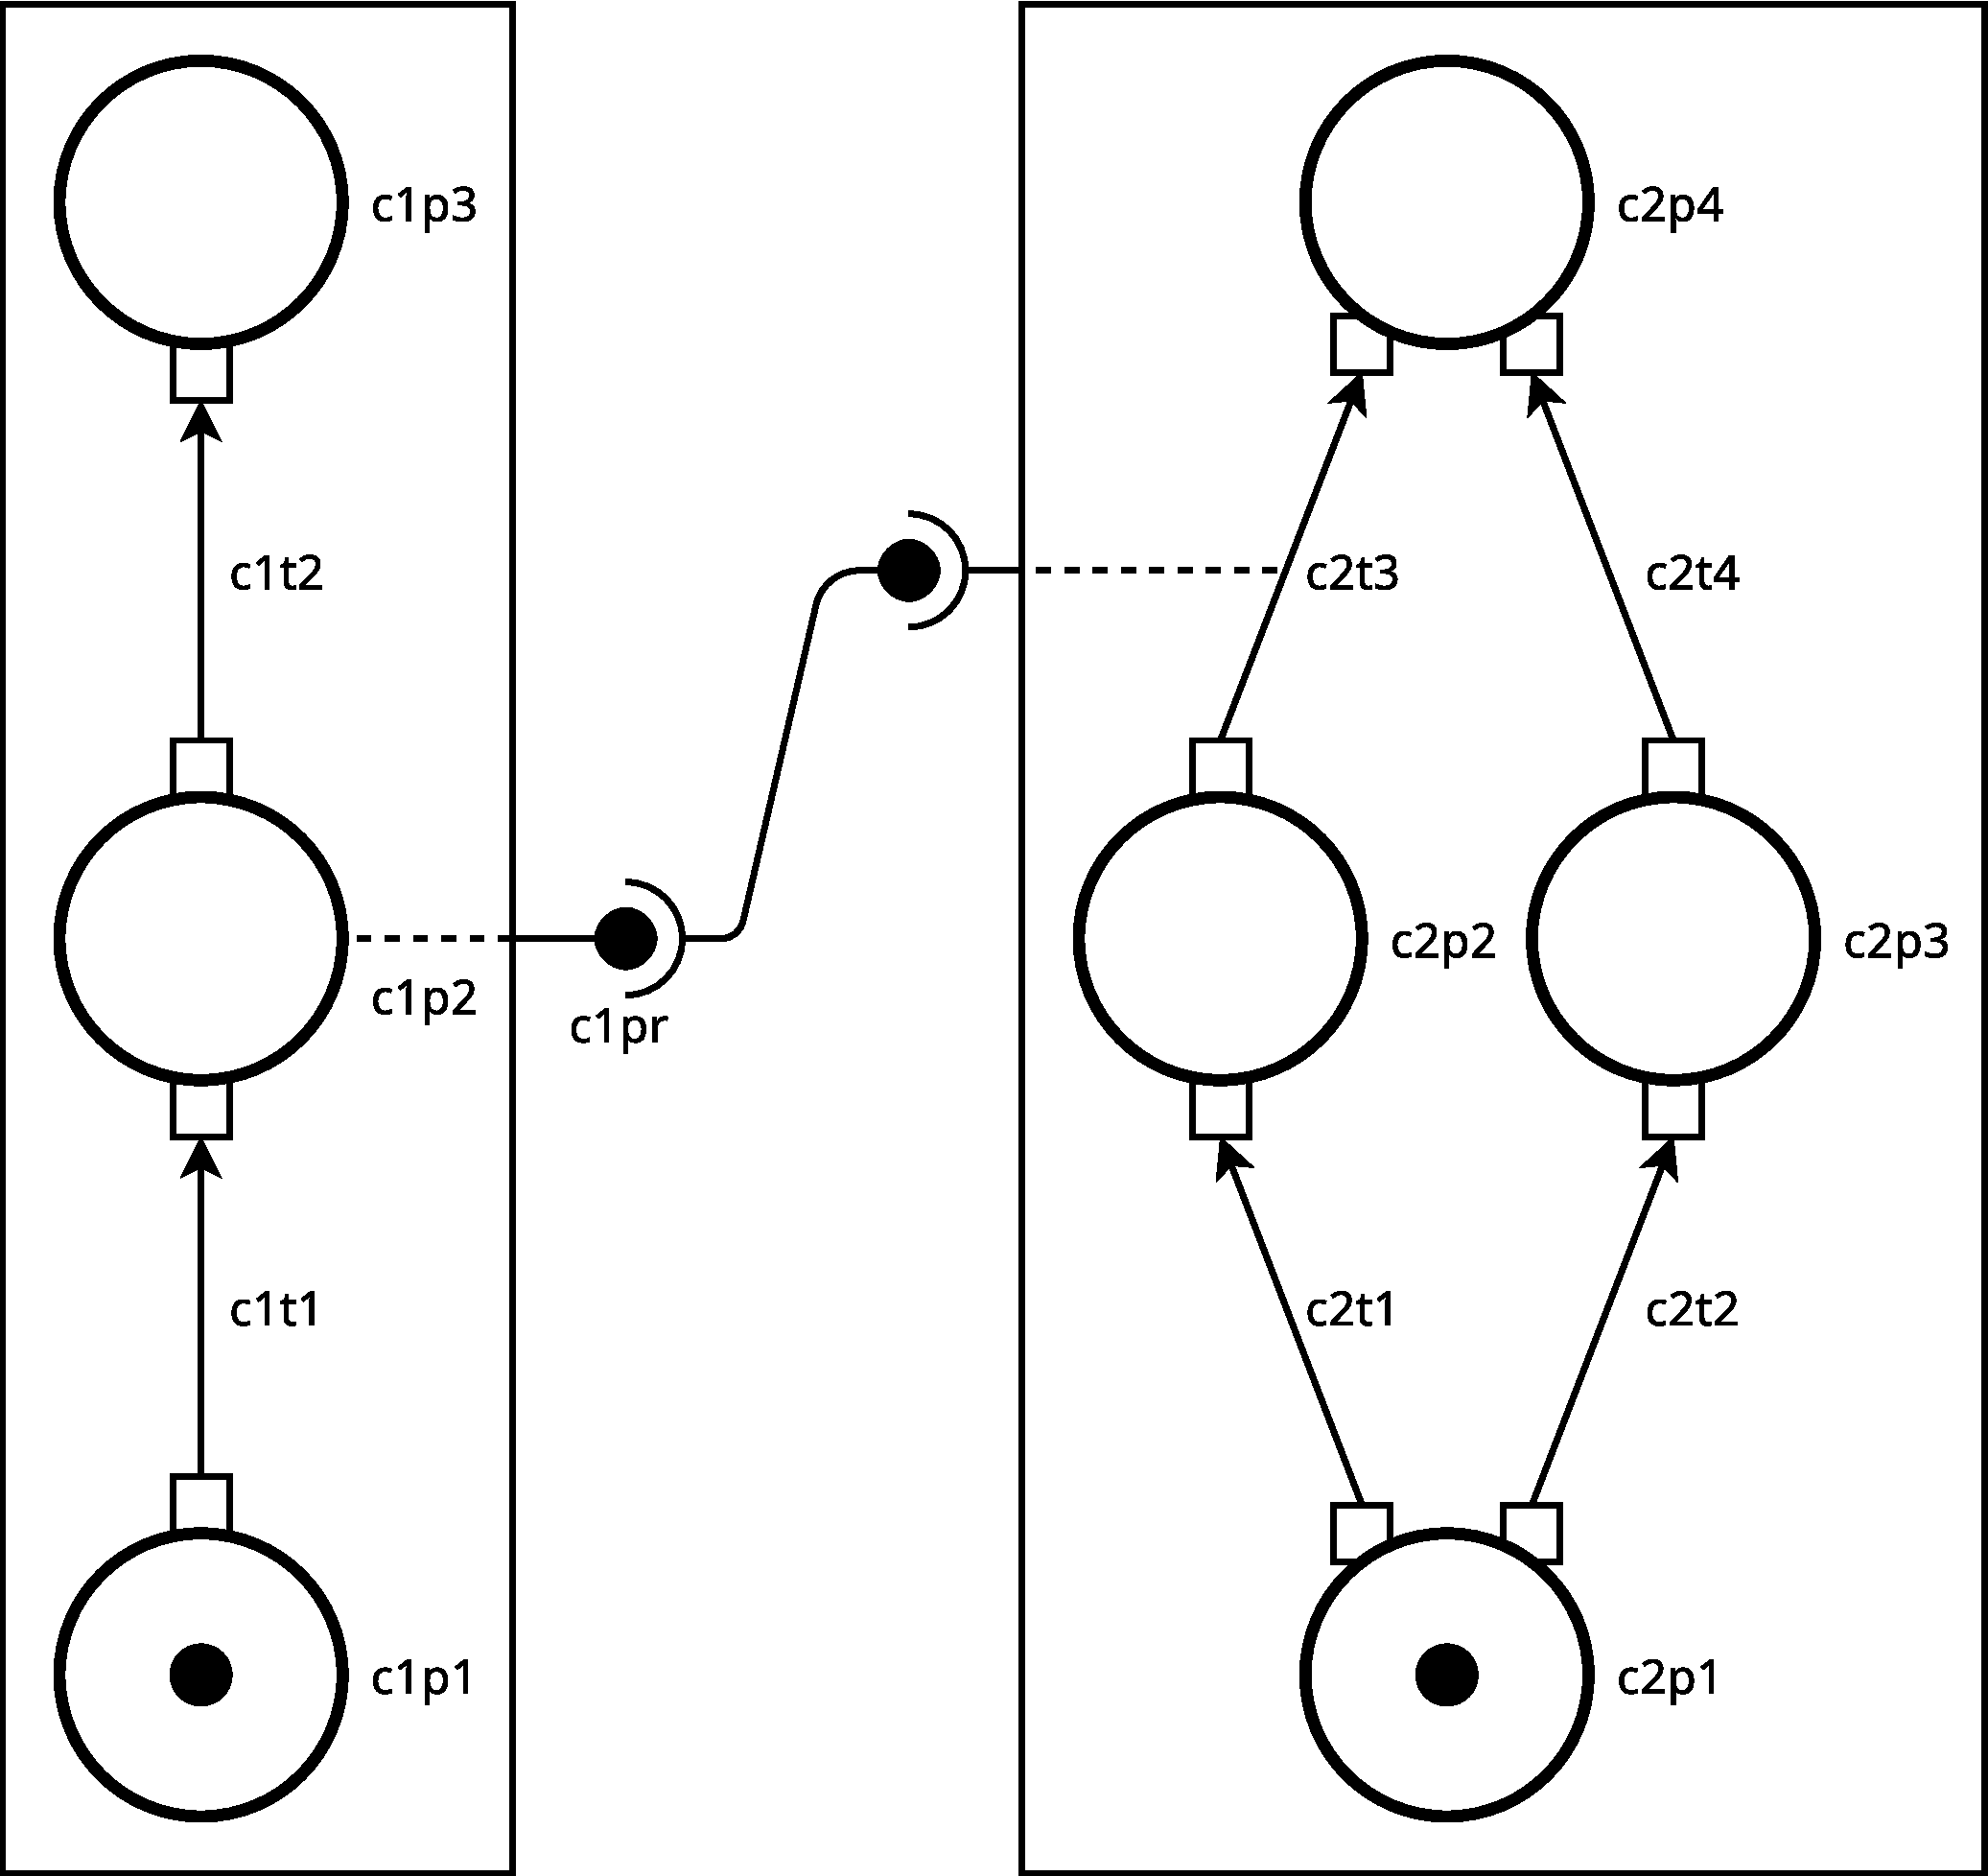
\includegraphics[scale=0.15]{images/perf_source_sink2.pdf}
    \end{minipage}
  }
  \\
  
  \subfloat[Dependency graph]{%
    \fcolorbox{black!20}{white}{
      \begin{minipage}[c]{0.95\columnwidth}%
        \centering
        \begin{tikzpicture}[node distance=1.7cm]
          \node (c1p3) [] {$v_\text{c1p3}^\text{reach}$};
          \node (c1t2) [below =15pt of c1p3] {$v_\text{c1t2}^\text{fire}$};
          \node (c1p2) [below =15pt of c1t2] {$v_\text{c1p2}^\text{reach}$};
          \node (c1t1) [below =15pt of c1p2] {$v_\text{c1t1}^\text{fire}$};
          \node (c1p1) [below =15pt of c1t1] {$v_\text{c1p1}^\text{reach}$};
          \node (c1pr) [right =30pt of c1p2] {$v_\text{c1pr}^\text{enable}$};
          \node (c2p2) [right =30pt of c1pr] {$v_\text{c2p2}^\text{reach}$};
          \node (c2t1) [below =15pt of c2p2] {$v_\text{c2t1}^\text{fire}$};
          \node (c2p1) [below =15pt of c2t1] {$v_\text{c2p1}^\text{reach}$};
          \node (c2t3) [above =15pt of c2p2] {$v_\text{c2t3}^\text{fire}$};
          \node (c2p4) [above =15pt of c2t3] {$v_\text{c2p4}^\text{reach}$};
          
          \node (c2p3) [right =30pt of c2p2] {$v_\text{c2p3}^\text{reach}$};
          \node (c2t2) [below =15pt of c2p3] {$v_\text{c2t2}^\text{fire}$};
          \node (c2t4) [above =15pt of c2p3] {$v_\text{c2t4}^\text{fire}$};
          
          \node (source) [below =81pt of c1pr] {$v^\text{source}$};
          \node (sink) [above =81pt of c1pr] {$v^\text{sink}$};
          
          \draw [->] (c1t1) -> (c1p2) node[midway, right, scale=0.7] {$t(\text{c1t1})$};
          \draw [->] (c1t2) -> (c1p3) node[midway, right, scale=0.7] {$t(\text{c1t2})$};
          \draw [->] (c2t1) -- (c2p2) node[midway, right, scale=0.7] {$t(\text{c2t1})$};
          \draw [->] (c2t2) -- (c2p3) node[midway, right, scale=0.7] {$t(\text{c2t2})$};
          \draw [->] (c2t3) -- (c2p4) node[midway, left, scale=0.7] {$t(\text{c2t3})$};
          \draw [->] (c2t4) -- (c2p4) node[midway, right, scale=0.7] {$t(\text{c2t4})$};
          \draw [->] (c1p1) -- (c1t1) node[midway, right, scale=0.7] {$0$};
          \draw [->] (c1p2) -- (c1t2) node[midway, right, scale=0.7] {$0$};
          \draw [->] (c2p1) -- (c2t1) node[midway, right, scale=0.7] {$0$};
          \draw [->] (c2p1) -- (c2t2) node[midway, below, scale=0.7] {$0$};
          \draw [->] (c2p2) -- (c2t3) node[midway, right, scale=0.7] {$0$};
          \draw [->] (c2p3) -- (c2t4) node[midway, right, scale=0.7] {$0$};
          \draw [->] (c1p2) -- (c1pr) node[midway, below, scale=0.7] {$0$};
          \draw [->] (c1pr) -- (c2t3) node[midway, below, scale=0.7] {$0$};
          \draw [->] (source) -- (c1p1) node[midway, below, scale=0.7]{$0$};
          \draw [->] (source) -- (c2p1) node[midway, below, scale=0.7] {$0$};
          \draw [->] (c1p3) -- (sink) node[midway, above, scale=0.7] {$0$};
          \draw [->] (c2p4) -- (sink) node[midway, above, scale=0.7] {$0$};
        \end{tikzpicture}
      \end{minipage}
    }
  }
  \caption{Two connected components and
    their equivalent dependency graph}
  \label{fig:source_sink_graph}
\end{figure}
